\documentclass[tikz, border=10pt]{standalone}
\usepackage{tikz}

\begin{document}

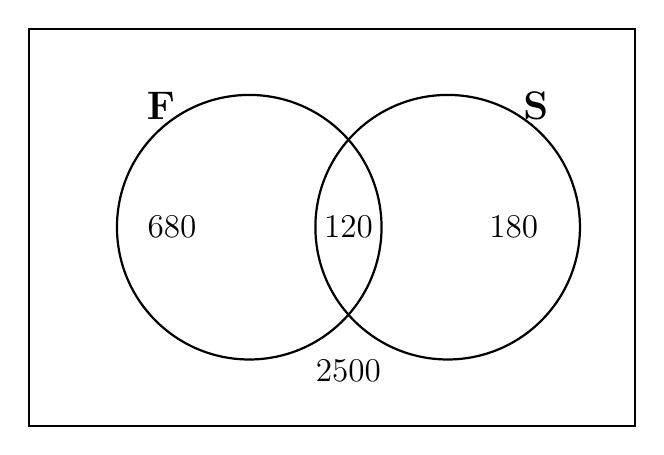
\begin{tikzpicture}[scale=1.4]
    % Draw the universal set rectangle (optional, can remove if not needed)
    \draw[thick] (-2,-1.8) rectangle (3.5,1.8);
    
    % Draw the two circles (outlines only)
    \draw[thick] (0,0) circle (1.2cm);
    \draw[thick] (1.8,0) circle (1.2cm);
    
    % Labels for the sets
    \node at (-0.8,1.1) {\Large \textbf{F}};
    \node at (2.6,1.1) {\Large \textbf{S}};
    
    % Numbers of students in each region
    % F ∩ S (both)
    \node at (0.9,0) {\large 120};
    % F only
    \node at (-0.7,0) {\large 680}; % 800 - 120
    % S only
    \node at (2.4,0) {\large 180}; % 300 - 120
    % Neither
    \node at (0.9,-1.3) {\large 2500}; % 3500 - 800 - 300 + 120 = 2500
\end{tikzpicture}

\end{document}
